\documentclass[12pt,aspectratio=169]{beamer}
% \hypersetup{pdfpagemode=FullScreen}

\usepackage{upgreek}
\usefonttheme{professionalfonts}

\renewcommand*{\thefootnote}{\fnsymbol{footnote}}

\mode<presentation>
\useoutertheme[subsection=false]{miniframes}

\title{vGraph: A Generative Model for Joint Community Detection and Node Representation Learning}
\author{Fan-Yun Sun\inst{1,2} \and %
        Meng Qu\inst{2} \and %
        Jordan Hoffmann\inst{2,3} \and %
        Chin-Wei Huang\inst{2,4} \and %
        Jian Tang\inst{2,5,6}}
\institute{\inst{1} National Taiwan University \and %
           \inst{2} Mila-Quebec Institute for Learning Algorithms, Canada \and %
           \inst{3} Harvard University, USA \and %
           \inst{4} Element AI, Canada \and %
           \inst{5} HEC Montreal, Canada \and %
           \inst{6} CIFAR AI Research Chair}
\date{Jul 13, 2020}

\begin{document}
    \beamertemplatenavigationsymbolsempty

    \makeatletter
    \def\beamer@andinst{\\[.1em]}
    \makeatother

    \begin{frame}
        \titlepage
    \end{frame}

    \section{Introduction}

    \begin{frame}
        \frametitle{Introduction}

        Graphs are a general and flexible data structure to encode complex relationships among objects. Examples of
        real-world graphs include social networks, airline networks, protein-protein interaction networks, and traffic
        networks. This paper focuses on two fundamental tasks of graph analysis: \textbf{community detection} and \textbf{node
        representation learning}, which capture the global and local structures of graphs, respectively.
    \end{frame}

    \begin{frame}
        \frametitle{Motivation}

        \centering
        \includegraphics[page=4,trim=6cm 8cm 0 1cm,clip,scale=0.6]{vGraph_slides.pdf}
        \includegraphics[page=4,trim=2cm 0 5cm 8cm,clip,scale=0.6]{vGraph_slides.pdf}
    \end{frame}

    \begin{frame}
        \frametitle{Motivation}

        \centering
        \includegraphics[page=5,trim=2cm 0 2cm 3cm,clip,scale=0.6]{vGraph_slides.pdf}
    \end{frame}

    \begin{frame}
        \frametitle{vGraph - probabilistic generative model}

        \begin{itemize}
            \setlength{\itemsep}{.8em}
            \item Generative model with Variational Inference to solve community detection and node representation learning jointly.
            \item Scalable: $O(d * |E| * K)$.
            \setbeamertemplate{itemize items}[circle]
                \begin{itemize}
                    \item $d$: embedding dimension
                    \item $|E|$: number of edges in the graph
                    \item $K$: number of communities
                \end{itemize}
            \setbeamertemplate{itemize items}[triangle]
        \end{itemize}
    \end{frame}

    \section{vGraph}

    \begin{frame}
        \frametitle{Problem Definition}

        Given a graph $G(V, E)$ where $V$ and $E$ represent the set of vertices and edges respectively, we aim to jointly
        learn a node embedding $\upphi_i \in \mathbb{R}^d$ and community affiliation $\mathcal{F}(\nu_i) \subseteq \{1, ..., K\}$
        for each vertex $\nu_i$.
    \end{frame}

    \begin{frame}
        \frametitle{Model}

        vGraph assumes that the edges $(w,c)$ is generated from the following stocastic process: for node $w$, we first
        draw a community assignment $z \sim p(z|w)$ representing the social context of $w$ during the generation process.
        Then, the linked neighbor $c$ is generated based on the assignment $z$ through $c \sim p(c|z)$. Formally, this
        process can be fomulated as:

        $$ p(c|w) = \sum_{z}{p(c|z)p(z|w)} $$
    \end{frame}

    \begin{frame}
        \frametitle{Model}

        \vskip -1em

        $$ p(c|w) = \sum_{z}{p(c|z)p(z|w)} $$

        \vskip 1em

        vGraph parameterizes the distributions $p(z|w)$ and $p(c|z)$ by introducing three sets of embeddings: $\upphi_i$,
        $\upvarphi_i$, and $\uppsi_j$. The prior distribution $p_{\upphi,\uppsi}(z|w)$ and the node distribution conditioned on
        a community $p_{\uppsi,\upvarphi}(c|z)$ are parameterized by two softmax models:

        $$ p_{\upphi,\uppsi}(z=j|w) = \frac{\exp(\upphi^T_w\uppsi_j)}{\sum^K_{i=1}\exp(\upphi^T_w\uppsi_i)} $$
        $$ p_{\uppsi,\upvarphi}(c|z=j) = \frac{\exp(\uppsi^T_j\upvarphi_c)}{\sum_{c\prime\in N}\exp(\uppsi^T_j\upvarphi_{c\prime})} $$
    \end{frame}

    \begin{frame}
        \frametitle{Variational Inference}

        The goal is to maximize the log-likelihood of the observed edges

        $$ \sum_{(c,w)\in E}\log{}p_{\upphi,\upvarphi,\uppsi}(c|w) $$

        Directly optimizing this objective is intractable for large graphs, we instead optimize the following evidence
        lower bound

        $$ \mathcal{L} = E_{z\sim q(z|c,w)}(\log p_{\uppsi,\upvarphi}(c|z)) - \mathop{KL}(q(z|c,w) \| p_{\upphi,\uppsi}(z|w)) $$

        where $q(z|c,w)$ is a variational distribution that approximates the true posterior distribution $p(z|c,w)$, and
        $\mathop{KL(\cdot\|\cdot)}$ represents the Kullback-Leibler divergence between two distributions.
    \end{frame}

    \begin{frame}
        \frametitle{Variational Inference}

        \vskip -1em

        $$ \mathcal{L} = E_{z\sim q(z|c,w)}(\log p_{\uppsi,\upvarphi}(c|z)) - \mathop{KL}(q(z|c,w) \| p_{\upphi,\uppsi}(z|w)) $$
        $$ p_{\upphi,\uppsi}(z=j|w) = \frac{\exp(\upphi^T_w\uppsi_j)}{\sum^K_{i=1}\exp(\upphi^T_w\uppsi_i)} $$
        $$ p_{\uppsi,\upvarphi}(c|z=j) = \frac{\exp(\uppsi^T_j\upvarphi_c)}{\sum_{c\prime\in N}\exp(\uppsi^T_j\upvarphi_{c\prime})} $$

        \vskip 1.5em

        Specifically, we parameterize the variational distribution using a neural network as follows ($\odot$ denotes element-wise multiplication):
        \vskip -.5em

        $$ q_{\upphi,\uppsi}(z=j|c,w) = \frac{\exp((\upphi_w \odot \upphi_c)^T\uppsi_j)}{\sum^K_{i=1}\exp((\upphi_w \odot \upphi_c)^T\uppsi_i)} $$
    \end{frame}

    \section{Implementation Details}

    \begin{frame}
        \frametitle{Straight-through Gumbel-Softmax estimator}

        It refactors the sampling operation into a deterministic function.

        $$ z = \mathop{argmax}_i\{{G_i + log(\pi_i)}\} $$

        where $G_i \sim Gumbel(0, 1)$. To pass gradients back, Straight-through estimator is used, which is basically using
        softmax to approximate the argmax operation during back propagation.
    \end{frame}

    \begin{frame}
        \frametitle{Community-smoothness Regularization}

        vGraph add the following regularization term to ensure that connected nodes tend to be in the same community:

        $$ \mathcal{L}_{reg} = \lambda\sum_{(w,c)\in E}\alpha_{w,c}\cdot d(p(z|c),p(z|w)) $$

        where $\lambda$ is a tunable hyperparameter, $d(\cdot,\cdot)$ is the distance measure (squared difference in the
        experiment). $\alpha_{w,c}$ is given by:

        $$ \alpha_{w,c} = \frac{\vert N(w) \cap N(c)\vert}{\vert N(w) \cup N(c)\vert} $$

        where $N(w)$ is the set of neighbors of $w$. The intuition behind this is that $\alpha_{w,c}$ serves as a
        similarity measure and the Jaccard's coefficient is used for this metric.
    \end{frame}

    \section{Experiments}

    \begin{frame}
        \frametitle{Experiment Setup}

        \begin{itemize}
            \setlength{\itemsep}{1.4em}
            \item 20 standard graph datasets.
            \item 3 tasks: overlaping community detection, non-overlaping community detection, and vertex classification.
        \end{itemize}
    \end{frame}

    \begin{frame}
        \frametitle{Overlapping community detection}

        \centering
        \includegraphics[page=6,trim=2.5cm 19.5cm 2.5cm 2cm,clip,scale=.8]{vGraph.pdf}
    \end{frame}

    \begin{frame}
        \frametitle{Non-overlapping community detection}

        \centering
        \includegraphics[page=7,trim=2.5cm 22cm 2.5cm 2cm,clip,scale=.8]{vGraph.pdf}
    \end{frame}

    \begin{frame}
        \frametitle{Vertex classification}

        \centering
        \includegraphics[page=7,trim=2.5cm 19cm 2.5cm 6cm,clip,scale=.8]{vGraph.pdf}
    \end{frame}

    \begin{frame}
        \frametitle{Visualization}

        \centering
        \includegraphics[page=8,trim=2.5cm 18.5cm 2.5cm 2cm,clip,scale=.8]{vGraph.pdf}
    \end{frame}

    \appendix

    \begin{frame}
        \frametitle{Conclusion}

        This paper presented a probabilistic method for jointly solving community detection and node representation
        learning. Experiments show that it performs well for both tasks.
    \end{frame}

    \begin{frame}
        \vskip 1.5em

        \centering \huge
        Thank you!
    \end{frame}
\end{document}
